\documentclass[12pt]{article}

%==============Packages & Commands==============
\usepackage{graphicx}
\usepackage{fancyvrb}
\usepackage{tikz}
%%%<
\usepackage{listings}
%\usepackage[active,tightpage]{preview}
%\PreviewEnvironment{tikzpicture}
%\setlength\PreviewBorder{5pt}%

\usepackage{geometry}                		% See geometry.pdf to learn the layout options. There are lots.
\geometry{letterpaper}                   		% ... or a4paper or a5paper or ...
%\geometry{landscape}                		% Activat\usetikzlibrary{arrows}e for for rotated page geometry
%\usepackage[parfill]{parskip}    		% Activate to begin paragraphs with an empty line rather than an indent
\usepackage{graphicx}				% Use pdf, png, jpg, or eps§ with pdflatex; use eps in DVI mode
								% TeX will automatically convert eps --> pdf in pdflatex
\usepackage{amsmath}
\usepackage{amssymb}

\usepackage[ruled,vlined]{algorithm2e}
\usetikzlibrary{arrows}
\usepackage{alltt}
\usepackage[T1]{fontenc}
%\usepackage[utf8]{inputenc}
\usepackage{indentfirst}
\usepackage[longnamesfirst]{natbib} % For references
\bibpunct{(}{)}{;}{a}{}{,} % Reference punctuation
\usepackage{changepage}
\usepackage{setspace}
\usepackage{booktabs} % For tables
\usepackage{floatrow}
\usepackage{rotating} % For sideways tables/figures
\usepackage{amsmath}
\usepackage{multirow}
\usepackage{color}
 
\definecolor{codegreen}{rgb}{0,0.6,0}
\definecolor{codegray}{rgb}{0.5,0.5,0.5}
\definecolor{codepurple}{rgb}{0.58,0,0.82}
\definecolor{backcolour}{rgb}{0.95,0.95,0.92}
 
\lstdefinestyle{mystyle}{
    backgroundcolor=\color{backcolour},   
    commentstyle=\color{codegreen},
    keywordstyle=\color{magenta},
    numberstyle=\tiny\color{codegray},
    stringstyle=\color{codepurple},
    basicstyle=\footnotesize,
    breakatwhitespace=false,         
    breaklines=true,                 
    captionpos=b,                    
    keepspaces=true,                 
    numbers=left,                    
    numbersep=5pt,                  
    showspaces=false,                
    showstringspaces=false,
    showtabs=false,                  
    tabsize=2
}
 
\lstset{style=mystyle}
\usepackage{dcolumn}
\usepackage{comment}
%\usepackage{fullwidth}
\newcolumntype{d}[1]{D{.}{\cdot}{#1}}
\newcolumntype{.}{D{.}{.}{-1}}
\newcolumntype{3}{D{.}{.}{3}}
\newcolumntype{4}{D{.}{.}{4}}
\newcolumntype{5}{D{.}{.}{5}}
\usepackage{float}
\usepackage[hyphens]{url}
%\usepackage[margin = 1.25in]{geometry}
%\usepackage[nolists,figuresfirst]{endfloat} % Figures and tables at the end
\usepackage{subfig}
\captionsetup[subfloat]{position = top, font = normalsize} % For sub-figure captions
\usepackage{fancyhdr}
%\makeatletter
%\def\url@leostyle{%
%  \@ifundefined{selectfont}{\def\UrlFont{\sf}}{\def\UrlFont{\small\ttfamily}}}
%\makeatother
%% Now actually use the newly defined style.
\urlstyle{same}
\usepackage{times}
\usepackage{mathptmx}
%\usepackage[colorlinks = true,
%						bookmarksopen = true,
%						pagebackref = true,
%						linkcolor = black,
%						citecolor = black,
% 					urlcolor = black]{hyperref}
%\usepackage[all]{hypcap}
%\urlstyle{same}
\newcommand{\fnote}[1]{\footnote{\normalsize{#1}}} % 12 pt, double spaced footnotes
\def\citeapos#1{\citeauthor{#1}'s (\citeyear{#1})}
\def\citeaposs#1{\citeauthor{#1}' (\citeyear{#1})}
\newcommand{\bm}[1]{\boldsymbol{#1}} %makes bold math symbols easier
\newcommand{\R}{\textsf{R}\space} %R in textsf font
\newcommand{\netinf}{\texttt{NetInf}\space} %R in textsf font
\newcommand{\iid}{i.i.d} %shorthand for iid
\newcommand{\cites}{{\bf \textcolor{red}{CITES}}} %shorthand for iid
%\usepackage[compact]{titlesec}
%\titlespacing{\section}{0pt}{*0}{*0}
%\titlespacing{\subsection}{0pt}{*0}{*0}
%\titlespacing{\subsubsection}{0pt}{*0}{*0}
%\setlength{\parskip}{0pt}
%\setlength{\parsep}{0pt}
%\setlength{\bibsep}{2pt}
%\renewcommand{\headrulewidth}{0pt}

%\renewcommand{\figureplace}{ % This places [Insert Table X here] and [Insert Figure Y here] in the text
%\begin{center}
%[Insert \figurename~\thepostfig\ here]
%\end{center}}
%\renewcommand{\tableplace}{%
%\begin{center}
%[Insert \tablename~\theposttbl\ here]
%\end{center}}

\newcommand\independent{\protect\mathpalette{\protect\independenT}{\perp}}
\def\independenT#1#2{\mathrel{\rlap{$#1#2$}\mkern2mu{#1#2}}}
\newcommand{\N}{\mathcal{N}}
\newcommand{\Y}{\bm{\mathcal{Y}}}
\newcommand{\bZ}{\bm{Z}}

\usepackage[colorlinks = TRUE, urlcolor = black, linkcolor = black, citecolor = black, pdfstartview = FitV]{hyperref}


%============Article Title, Authors==================
\title{\vspace{-2cm} Experiments on Interactive Groups, and Network Effects: Examples from Legislative Studies } 


\author{Sayali Phadke \thanks{\footnotesize{PhD Student, Departments of Statistics, Pennsylvania State University, ssp5208@psu.edu.}} \and Bruce A. Desmarais \thanks{\footnotesize{Associate Professor, Department of Political Science, Pennsylvania State University, bdesmarais@psu.edu.}}} \date{\today}



%===================Startup=======================
\begin{document}
\maketitle



%=============Abstract & Keywords==================

\begin{abstract} 
\vspace{.3cm}
\begin{center}
{\bf DRAFT, RESULTS MAY CHANGE}
\end{center}
\vspace{.3cm}

\noindent  Most social processes involve complex interaction among units through some form of social, communication, or collaboration network. The stable unit treatment value assumption (SUTVA)---the assumption that a unit's outcome is unaffected by other units' treatment statuses---is required in conventional approaches to causal inference. When SUTVA is violated, as in networked social interaction, treatment effects spread to control units through the network structure. We evaluate the evidence for spillover effects in data from three field experiments on US state legislatures. Randomized field experiments represent the gold standard in causal inference when studying political elites. It is rarely possible to bring political elites into a controlled laboratory environment, and causal identification with observational data is fraught with problems. We review recently-developed methods for testing for causal effects---including interference effects---while relaxing SUTVA. We propose new specifications for treatment spillover models, and construct networks through geographical or ideological proximity and co-sponsorship. Considering different combinations of spillover models and networks, we evaluate the robustness of recently developed non-parametric tests for interference. The approaches we illustrate can be applied to any experimental setting in which interference is suspected. 

\end{abstract}

\thispagestyle{empty}
\doublespacing

% Description of the possible challenges
\section{Introduction}

In social science, researchers often focus on sets of actors who interact on a regular basis. Areas of social science research in which regular and familiar interaction constitutes the norm include the study of team performance in formal organizations \citep[e.g., ][]{anderson1992}, the study of students from the same school/classroom \citep[e.g., ][]{sallis1997}, and the study of political elites from the same political institution \citep[e.g.,][]{bratton1999}. The importance of collections of highly interactive individuals, which may have conventionally been termed ``small groups.'' \citep{levine1990}, spans disciplines; including social psychology, public health, political science and organizational studies. Given the rise of research focused on social media \citep{agichtein2008}, which includes the study of interpersonal interaction, but is focused on large groups, we will use the term, ``interactive group research.'' 

To draw causal inferences in the study of an interactive group, the most reliable approach is to run a randomized experiment in which the researcher controls one or more interventions. Due to the interactions between group members, the effect of an intervention on one group member may spread to others through the network of interactions. The conventional framework for causal inference relies on SUTVA (Stable Unit Treatment Value Assumption). SUTVA holds that one unit/subject is not affected by the treatment status of any other unit \citep{sekhon2008}. However, SUTVA breaks down in a network setting \citep{galea2010} when there are post-treatment interactions among units. The violation of SUTVA is termed ``interference''.  When testing for causal effects in experiments on interactive groups, there are two related motivations for researchers to test and account for interference. First, even if the researcher is not interested in the nature of interference, it may be necessary to account for interference to accurately identify the direct effects of interventions on units. Second, interference processes may play a major role in shaping individual or group outcomes, and may therefore be important to evaluate if the objective of the research is to understand or explain outcomes arising from the group's social process. 

ocial influence and other processes of interdependence are central to nearly every domain of social science, researchers are well aware of the major limitations associated with causal inferences regarding influence drawn from observational studies \citep{Shalizi:2011}. As such, a growing body of research seeks to study interference through experimental interventions \citep[e.g., ][]{gerber2008,paluck2011,Bond:2012,muchnik2013,aral2014,bapna2015,Ben-AaronPAR}. These studies follow a variety of approaches to designing the interventions and testing for interference effects. However, it is clear that the field has, as of yet, converged upon a consistent methodological framework for testing for causal effects in the presence of interference.  

We review a recently developed general framework, introduced by \citet{bowers2012reasoning}, for testing causal hypotheses in the presence of interference. As an illustration, we then apply this methodology to data generated by field experiments on US state legislatures \citep{butler2011can,bergan2015call}; experiments that were not intended to study interference. As part of our application, we discuss and illustrate several choices researchers need to make in testing interference hypotheses.

Our results are three-fold. First, we review a broad framework for evaluating interference hypotheses, and make the case that researchers should consider such hypotheses when evaluating the results of experiments on interactive groups. Second, we show that we consistently find evidence in support of interference hypotheses in data from field experiments on US state legislatures. Third, we encourage researchers to consider several modeling dimensions in formulating interference hypotheses.

%\section{Background}

%\begin{itemize}
%\item Paragraph on each category of papers that serve as relevant background (SP)
%\item Interference models (diffusion, propagation) (SP--Review)
%\item  Experiments on networks (applications) (SP--Review)
%\item Approaches to inference or estimation with propagation (SP--Review) 
%\item Potential outcomes framework (SP -- find papers \& Review)
%\item Review of political networks (SP--Review)
%\item Review of field experiments (SP--Review)
%\begin{itemize}
%\item \citep{Gottlieb:2015,Alatas:2012,Kalla:2015, Malesky:2012,Ichino:2012,Nyhan:2014}
%\end{itemize}
%\end{itemize}




\section{Research Design}

We intend to to re-analyze data from past field experimental studies to understand how conclusions regarding direct effects and interference effects depend upon the network structure. Several key factors must be considered while building a propagation models.


\begin{enumerate}
\item Distance from the nearest treated node ($d_i$)
\item Number/proportion of treated nodes neighboring each $d_i$
\item Form of spread (linear or non-linear)
\end{enumerate}


Table 1 tabulates the basic idea of the models we will look at. The linear/non-linear refers to the form taken by the spread of effect. Distance from the nearest treated node is temporarily separated as <5 or >5. Finally, we want to look at the difference in spillovers effects caused due to number of treated neighbors as against proportion of treated neighbors. Potentially, the number/proportion at hops of different lengths can also be considered.


\floatsetup[table]{objectset=centering,capposition=top}
\begin{table}
        \begin{tabular}{lrrrr}\toprule
            &\multicolumn{2}{c}{\textbf{Distance from treated < 5}}&\multicolumn{2}{c}{\textbf{Distance from treated > 5}}
            \\\cmidrule(r){2-3}\cmidrule(r){4-5}
            &Linear&Non-linear&Linear&Non-linear\\\midrule
            Number of treated neighbors    & 1 & 2
                    & 5 & 6\\
            Proportion of treated neighbors   & 3 & 4
                    & 7 & 8
            \\\bottomrule
        \end{tabular}
        \caption{Rough sketch of the several models considered}\label{Tab2}
\end{table} 


The types of networks we will consider in the analysis are:

\begin{enumerate}
\item Geographical proximity
\item Ideological similarity
\item Co-sponsorship
\end{enumerate}

Each of these factors is such, that the treatment would possibly spread to untreated units as well. Legislators from adjoining districts may affect each other's opinions through geographic proximity as well as potentially via common issues faced by citizens in their constituencies.

Ideological similarity can be hard to distinguish that from party affiliation. However, similar ideological scores can indicate similarity in ideas and belief about citizen's issues and how to resolve them. It would be very easy to affect thoughts of untreated neighbor in the ideological network.

Finally, serving on the same committee can also contribute to spreading the effect of a treatment. We must test for any dependence across these three factors before incorporating them into our model. Therefore it is important that we propose and test propagation models that consider the spread of treatment through our network.




\section{Analysis}

We begin this section by reviewing prior methodological work. We will look at two spillover specifications and testing frameworks given in \citet{bowers2012reasoning} and \citet{coppock2014information} papers. We will extend their analysis by considering various other specifications for spillover effects. Additionally, we intend to look into tests other than the Kolmogorov-Smirnov (KS) test.

\subsection{Review of existing methods}
\begin{itemize}
\item {\bf Bowers et. al. method:} This paper introduces a Fisherian inference algorithm to test for spillover of treatment effect. The model $\mathcal{H}$ is compared against the observed data. The hypothesized model of interference is specified by the researcher. The steps involved in conducting this test are as follows:

\begin{enumerate}

\item Assume the "sharp null hypothesis of no effects" i.e. the treatment assignment has no effect on any unit

\item Specify the causal model which describes the change in potential outcomes when treatment assignment changes from \textbf{u} to \textbf{w}; $\mathcal{H}(y_{i, \textbf{u}}, \textbf{w}, \theta)$

\item Potential outcomes from the causal model must be mapped to observed outcomes $y_z$. Treatment assignment in the experiment (\textbf{z}) must be mapped to the uniformity trial ($\mathcal{H}(y_{\textbf{z}}, \textbf{0}, \theta) = \textbf{y}_0$) which is based on the baseline condition of no-treatment assignment i.e. every unit is a control unit

\item Test statistic $\mathcal{T}$ should be a small value when distribution of treated and control outcomes in the adjusted data are similar, and a large value when distributions are dissimilar. We need a sensitive measure to account for similarity on not just the center but also higher-order moments of a distribution. \citet{bowers2012reasoning} recommend the Kolmogorov-Smirnov (KS) test statistic

\item Assume that treatment only spreads through edges and the spillover effect only depends on the number of neighbours treated. Spillover effect modeled using a growth curve $\beta + (1-\beta)e^{-\tau^2\textbf{z}^T\textbf{S}}$

\item Generate the distribution of test statistic under our hypothesis. The exact distribution is specified by computing $t_k = \mathcal{T} (\textbf{y}_0, \textbf{Z}_k)$ for each $\textbf{Z}_k \in \Omega$. Alternatively, we can use sampling methods and limit theorems to estimate the distribution from data.

\item p-value calculated using $\frac{\sum_{k=1}^{|\Omega|} I(x_i  > t_k)}{|\Omega|}$

\end{enumerate}

The user-defined R-function for this method is available in Appendix 1A.

\item {\bf Coppock replication:} Coppock builds upon the New Mexico Legislator experiment conducted by \citet{butler2011can}. This paper also works with the idea of sharp null of no effects and uniformity trial. Similarity in ideological scores is used as the adjacency matrix. The key difference between the two methods is that the Bowers method can only be applied to datasets which have continuous outcomes. This methods extends the framework for dichotomous outcome. Procedure is as follows:

\begin{itemize}

\item W-NOMINATE ideology score calculated for each legislator using rollcall vote data

\item Ideological similarity calculated as $Similarity_{i,j} = \frac{2 - |ideo_i - ideo_j|}{2}$

\item Raw exposure calculated as $Raw exposure_i =  \sum_{j=1}^{n}Similarity_{i,j} * z_j, j \neq i$. However, this specification introduces a correlation between exposure - direct treatment, exposure - ideology and exposure - other unobservable characteristics. Therefore we further process the raw exposures.

\item To calculate expected exposures, we simulate exposures under a large number of randomizations. Each randomization where legislator \textit{i} is in treatment is indexed as \textit{k} (\textit{k} = 1, 2, ..., K) and where legislator \textit{i} is in control is indexed as \textit{l} (\textit{l} = 1, 2, ..., L) $$Expected exposure_{i, z_i=1} =  \frac{\sum_{k=1}^{K}\sum_{j=1}^{n}Similarity_{i,j} * z_{j,k}}{K}, j \neq i, z_{i,k}=0$$ $$Expected exposure_{i, z_i=0} =  \frac{\sum_{l=1}^{L}\sum_{j=1}^{n}Similarity_{i,j} * z_{j,l}}{L}, j \neq i, z_{i,l}=1$$

\item Using ideological similarity scores in the adjacency matrix, Coppock separates out the direct treatment effect and spillover occurring through the network.

\end{itemize}

The user-defined R-function for this method is available in Appendix 1B.

\end{itemize}


\subsection{Extensions of Coppock analysis}

We consider several extensions of the Coppock method, applied to both datasets depending on availability of data.

\begin{itemize}

\item Consider k (=3, 5, 8, 12) neighbors according to ideological scores to form adjacency matrix. A tie between i and j indicates that legislator j is one of the k-nearest neighbors to i. This generates some ties. We will try the following two ways of taking care of the ties:

\begin{enumerate}
\item Choose, among the ties in the k closest neighbors for i, those nodes for which i is the closest neighbor. To illustrate, if i is equally close to j and h, we ask whether i ranks higher on j's list of closest neighbors. If yes, then we take out h. If no, we keep j and h if i ranks equally on j and h's neighbor list, or kick out j if h ranks i more highly.

\item Look at the number of nodes for which j is the nearest neighbor and in some way account for the j's influence on that basis
1. Look at control unit i
2. Calculate a composite score that indicates the ranking of i for each of its k neighbors
3. Estimate a parameter to see if change in composite score leads to a change in propensity for changing the outcome
4. This parameter will be modeled as a non-linear effect

For example, say k=3 condition. If a control unit is the lowest in the proximity of all of its 3 neighbors, it is less likely to receive a spillover; as compared to if it was in the highest proximity of all three of them (the two extremes). We would have to condition this on the treatment status of its neighbors.
\end{enumerate}

\item Consider committee network instead of ideological network, where a tie between i and j indicates that they have served on two or more committees together

\item Use number of shared committees in adjacency matrix

\item Separate out the high and low support district in original \citet{butler2011can} data and conduct separate analyses. This would explain the direction of the spillover effect much better. Conduct this analysis with ideological network as well as committee network

\item Include geographical network in both dataset and extend analysis

\item Consider various spillover models other than the growth curve specification

\item Consider weighted combinations of different networks to estimate a $\gamma$

\item Explore the idea of using communities to model spread across the network

\end{itemize}


\subsection{Results}
In this section we present results of data analysis for both datasets, in form of p-value plots. These p-values are the proportion of permutation tests whose test statistic is more extreme (greater or lesser depending on test) than the observed test statistic. Therefore higher p-values indicate departure from the null hypothesis of uniformity trial, providing evidence of spillover effect.

\subsubsection{Results for \citet{butler2011can} data}

The data for this replication was obtained from the publicly available data repository created by the authors. Records of standing committee membership in the 16 standing committees in place during the 2008 regular session was obtained from the New Mexico Legislative Council Service Librarian.

P-value plot of replication of the main analysis is in figure 1. Here we observe negative direct and indirect effects to have the highest p-values.
\begin{figure}
	\centering
	\begin{tabular}{cc}
	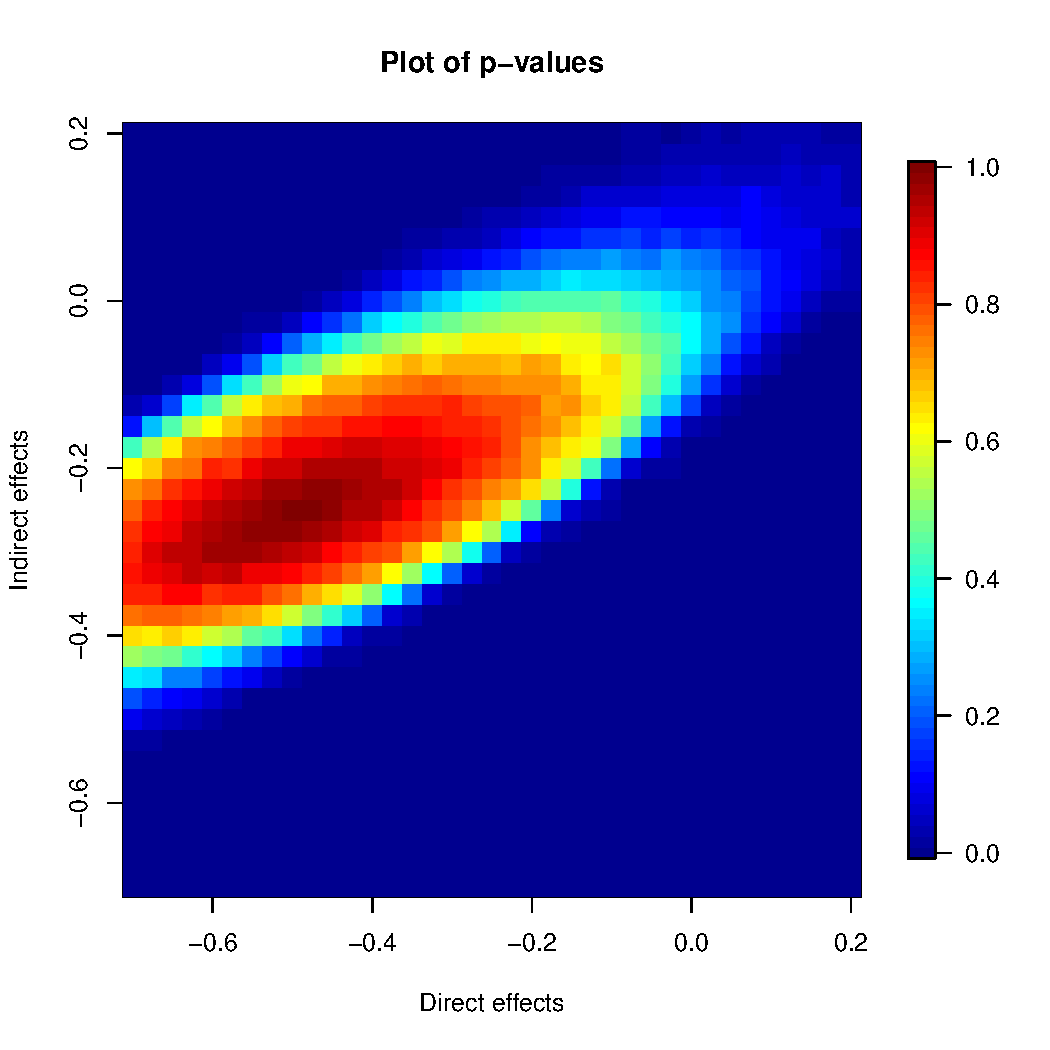
\includegraphics[scale=0.5]{./images/pvalues_figure_Coppock.pdf}
	\end{tabular}
	\caption{p-values: main analysis for \citet{butler2011can} data}
\end{figure}


As a first extension, we consider k-nearest neighbors based on ideological similarity (k = 3, 5, 8 12). In these plots (figure 2), highest values move closer to zero value for both effects, indicating low spillover as well as direct effect based on nearest ideological neighbors.
\begin{figure}
	\centering
	\begin{tabular}{cc}
	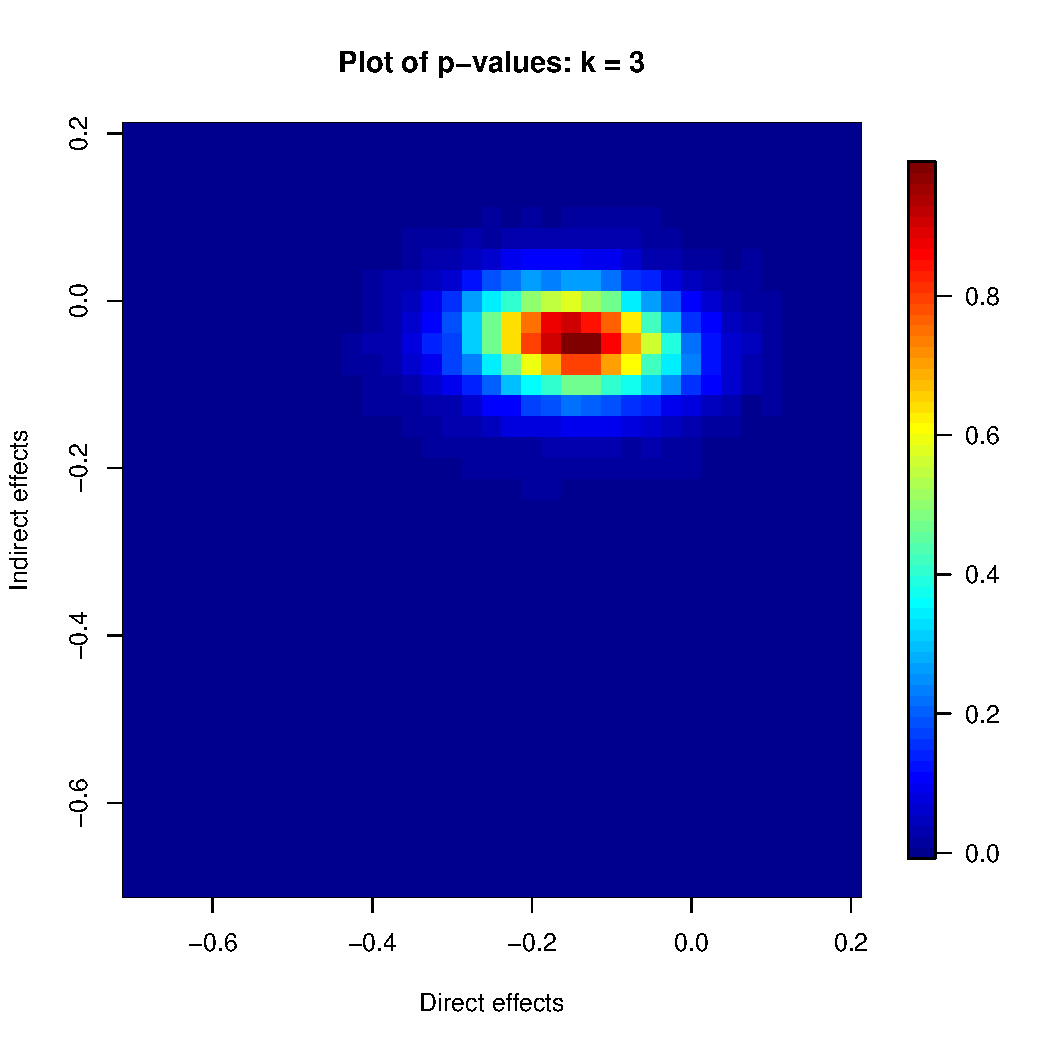
\includegraphics[scale=0.45]{./images/pvalues_figure_3nn_Coppock.pdf} &
	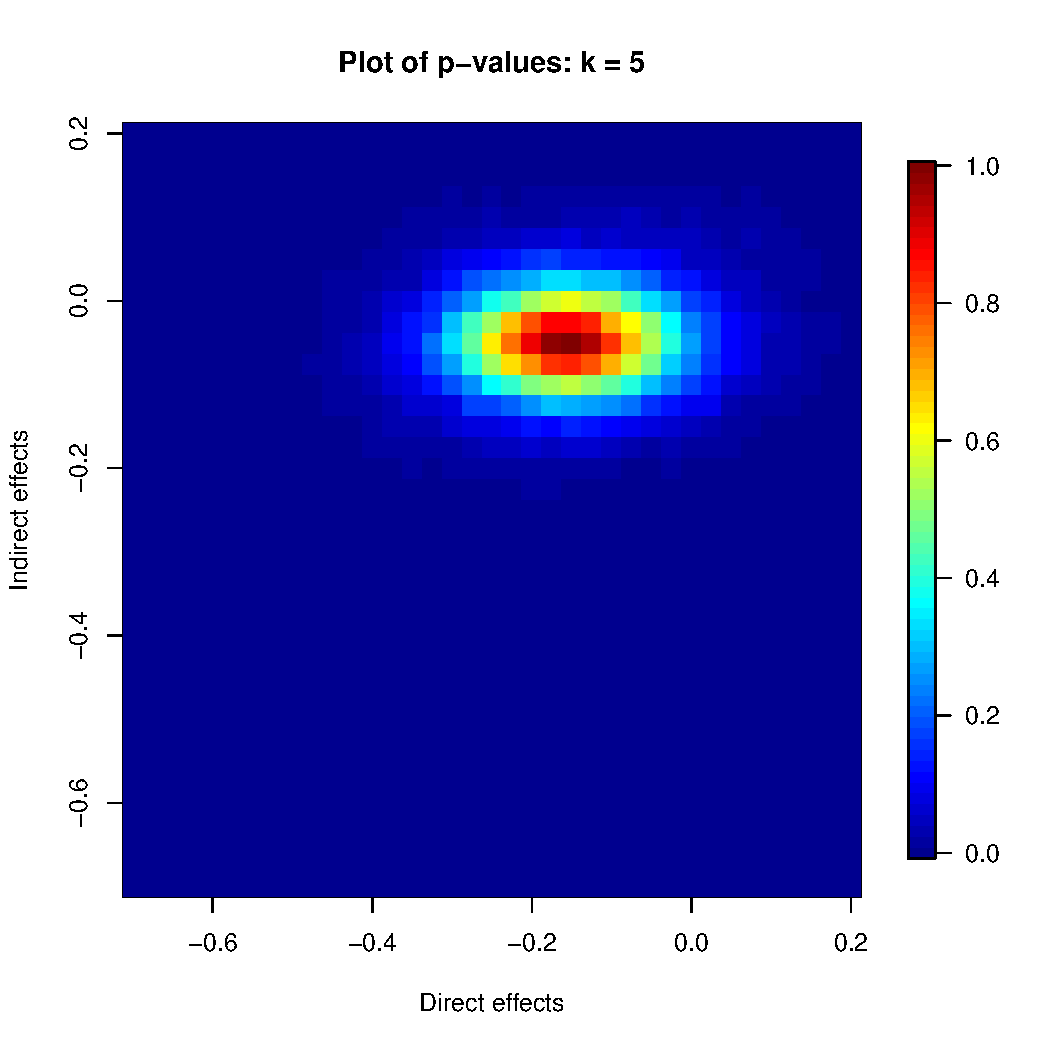
\includegraphics[scale=0.45]{./images/pvalues_figure_5nn_Coppock.pdf} \\ 
	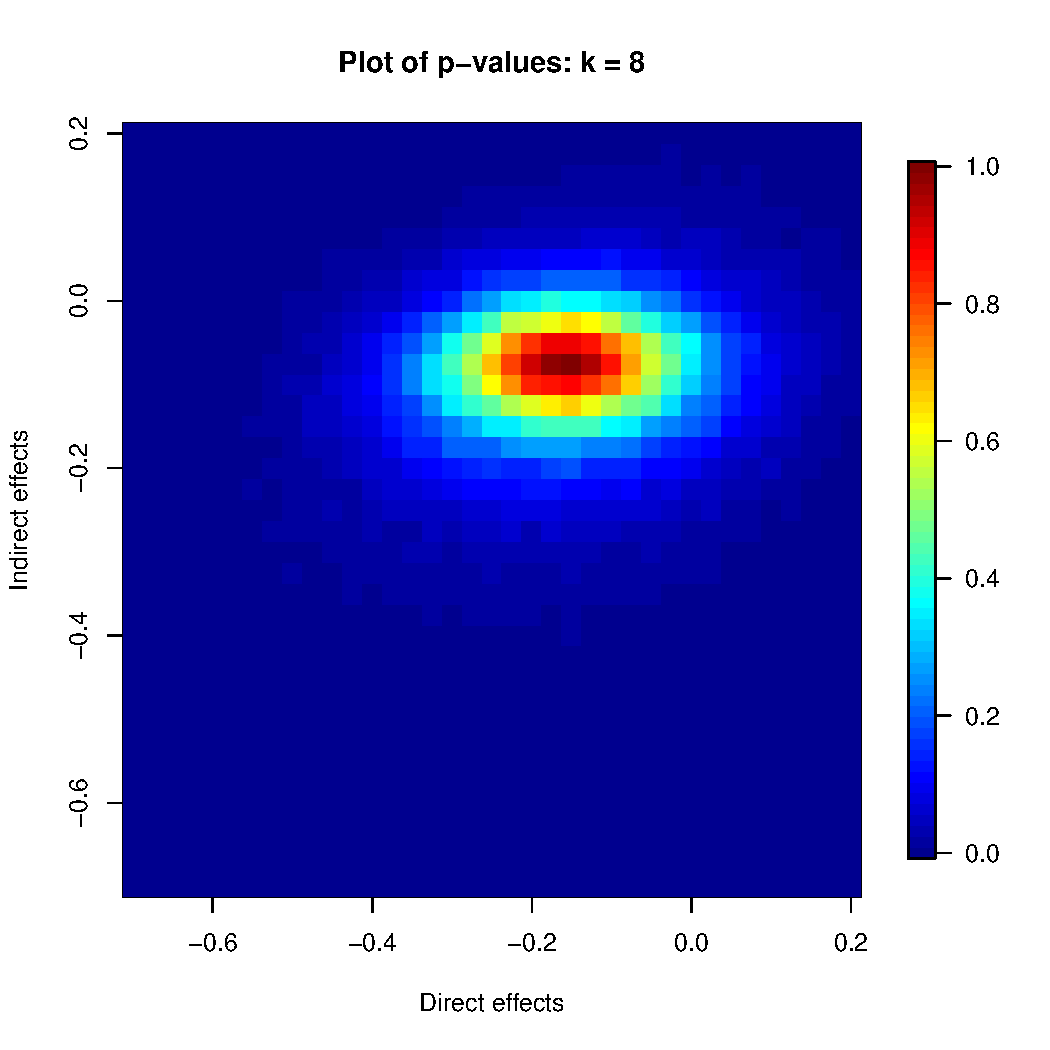
\includegraphics[scale=0.45]{./images/pvalues_figure_8nn_Coppock.pdf} &
	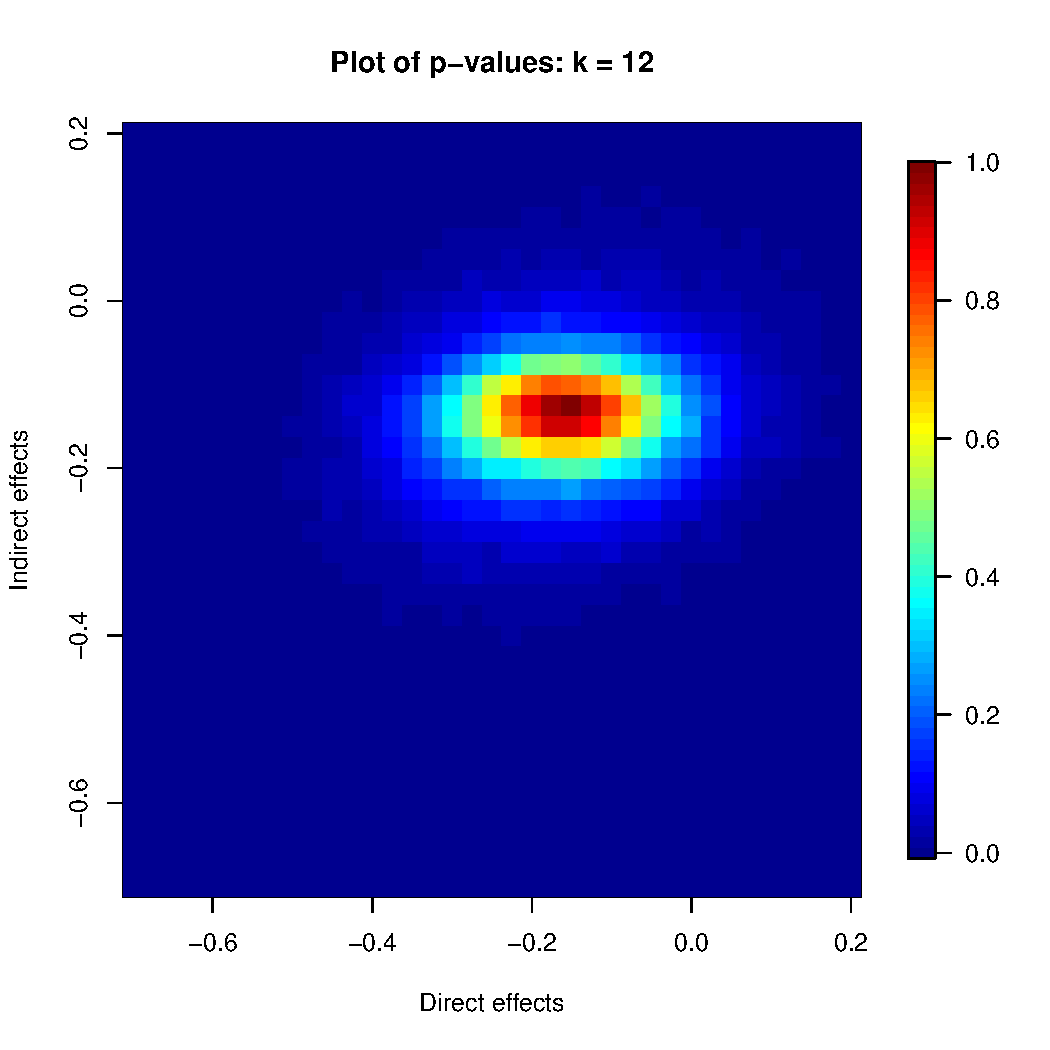
\includegraphics[scale=0.45]{./images/pvalues_figure_12nn_Coppock.pdf} \\ 
	\end{tabular}
	\caption{p-values: k-nearest neighbors for \citet{butler2011can} data}
\end{figure}


Second extension of this analysis considers committee network instead of ideological network. Here, an undirected tie exists between legislators who have served on two or more legislative committees together. We see in figure 3 that there is no evidence of spillover effect based on whether legislators have served on legislative committees together or not.
\begin{figure}
	\centering
	\begin{tabular}{cc}
	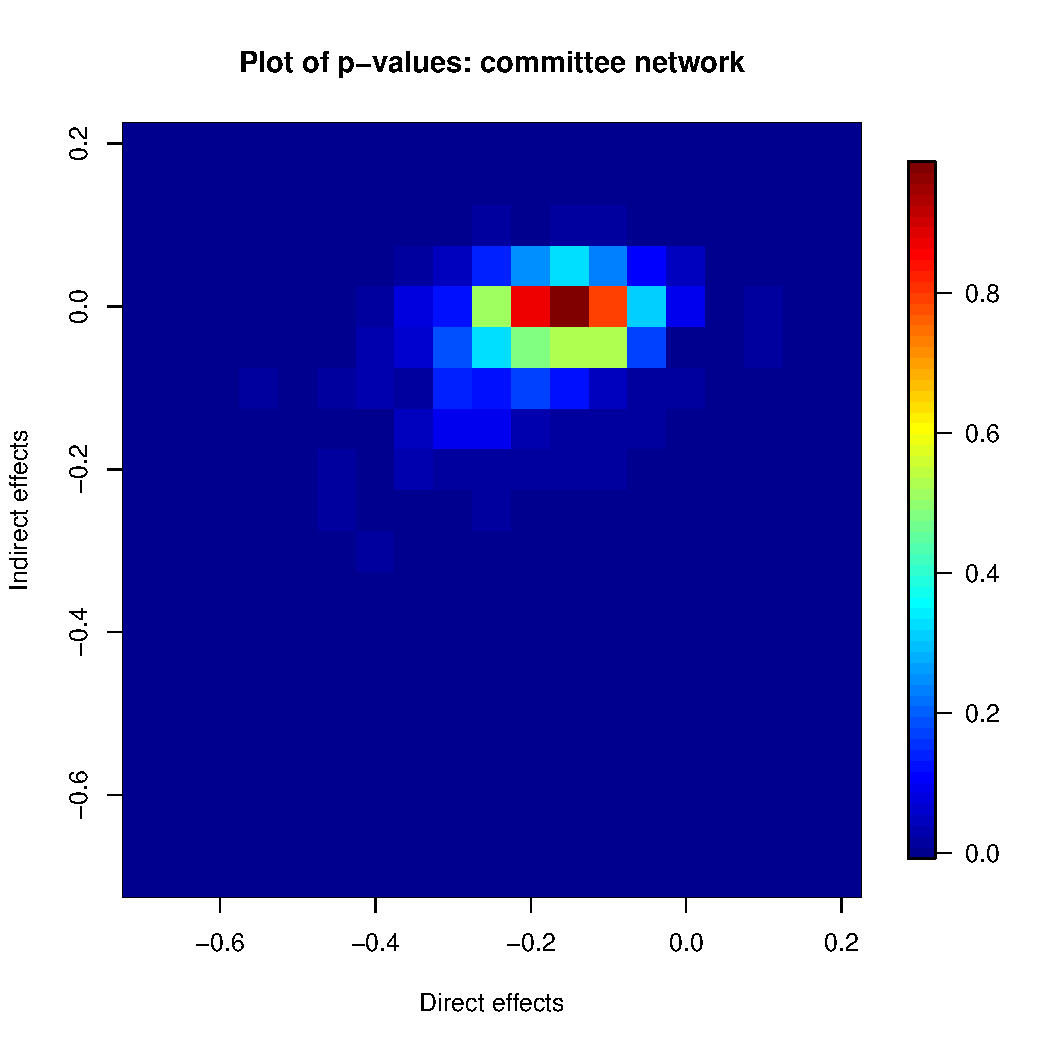
\includegraphics[scale=0.5]{./images/pvalues_figure_committee_at_least_one_Coppock.pdf}
	\end{tabular}
	\caption{p-values: main analysis for \citet{butler2011can} data}
\end{figure}


In the currently available final extension, we use the committee network but a tie here indicates the number of committees on which legislators have served together. This analysis (figure 4) does not show evidence of spillover effect either.
\begin{figure}
	\centering
	\begin{tabular}{cc}
	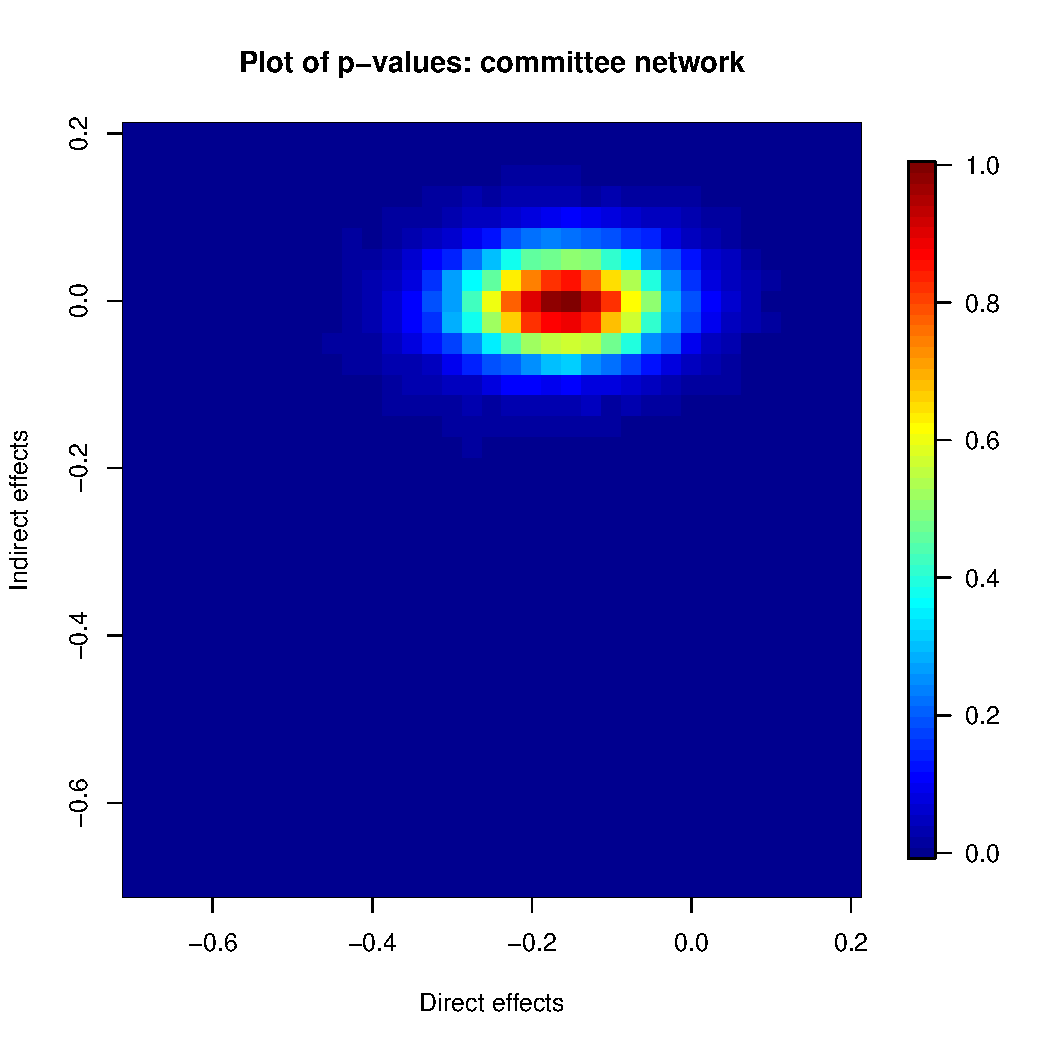
\includegraphics[scale=0.5]{./images/pvalues_figure_committee_Coppock.pdf}
	\end{tabular}
	\caption{p-values: main analysis for \citet{butler2011can} data}
\end{figure}




\subsubsection{Results for \citet{bergan2015call} data}

We begin by looking at the p-value plot of analysis using the main setup where adjacency is based on similarity of ideology scores calculated using rollcall vote data. Here, we see that the highest p-value is close to 0.1 for both direct and indirect effect
\begin{figure}
	\centering
	\begin{tabular}{cc}
	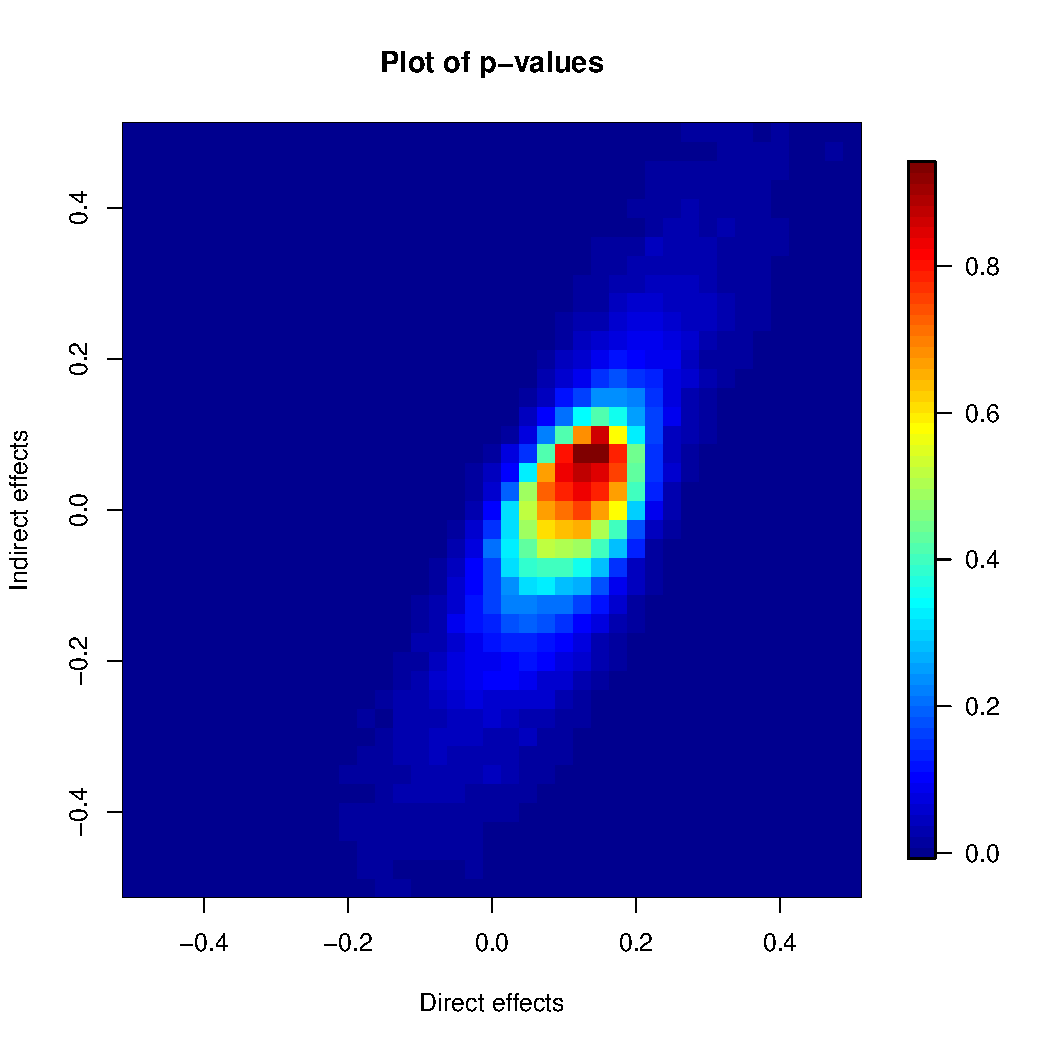
\includegraphics[scale=0.5]{./images/pvalues_figure_main_Bergan.pdf}
	\end{tabular}
	\caption{p-values: main analysis for \citet{bergan2015call} data}
\end{figure}


Figure 6 extends this analysis to consider k-nearest ideological neighbors, as earlier. We see no evidence of spillover effect in these plots.
\begin{figure}
	\centering
	\begin{tabular}{cc}
	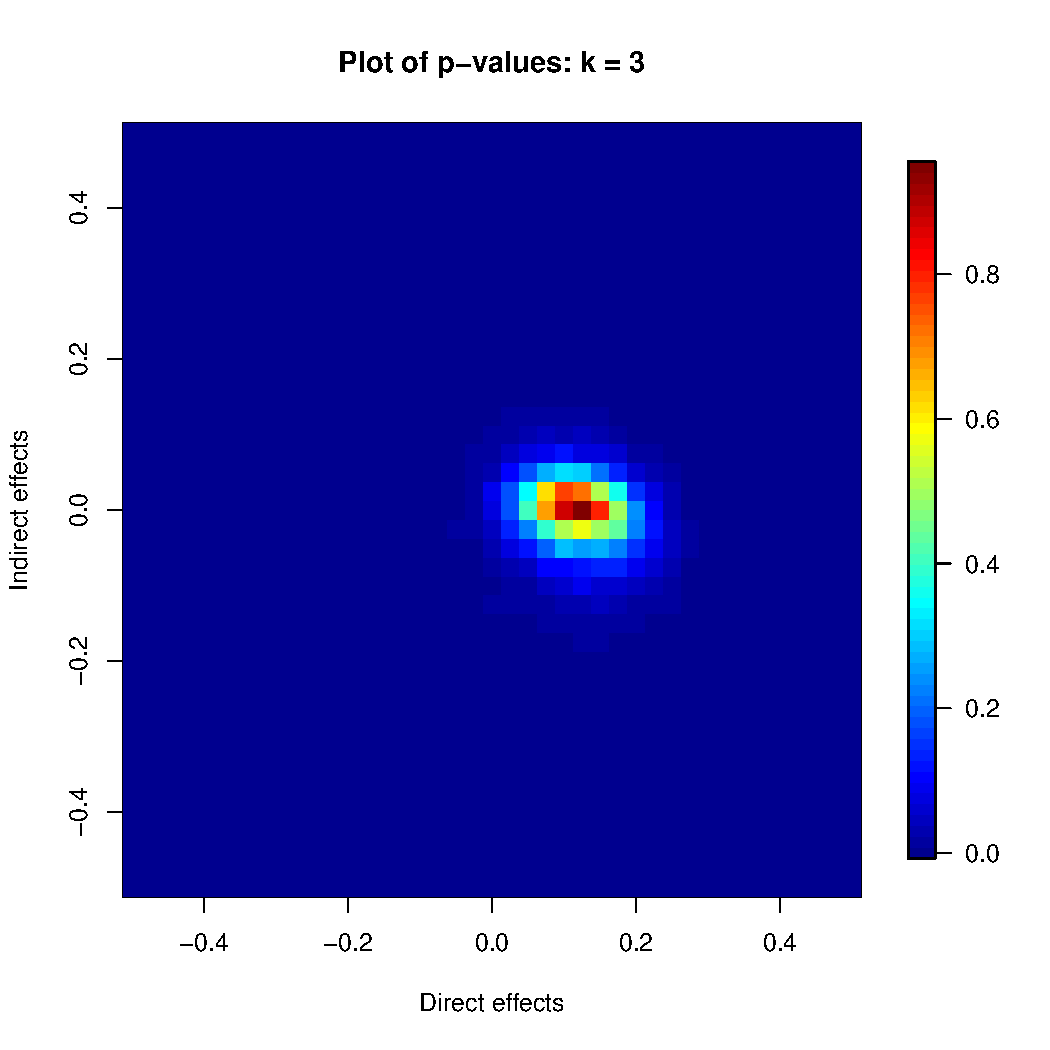
\includegraphics[scale=0.45]{./images/pvalues_figure_3nn_Bergan.pdf} &
	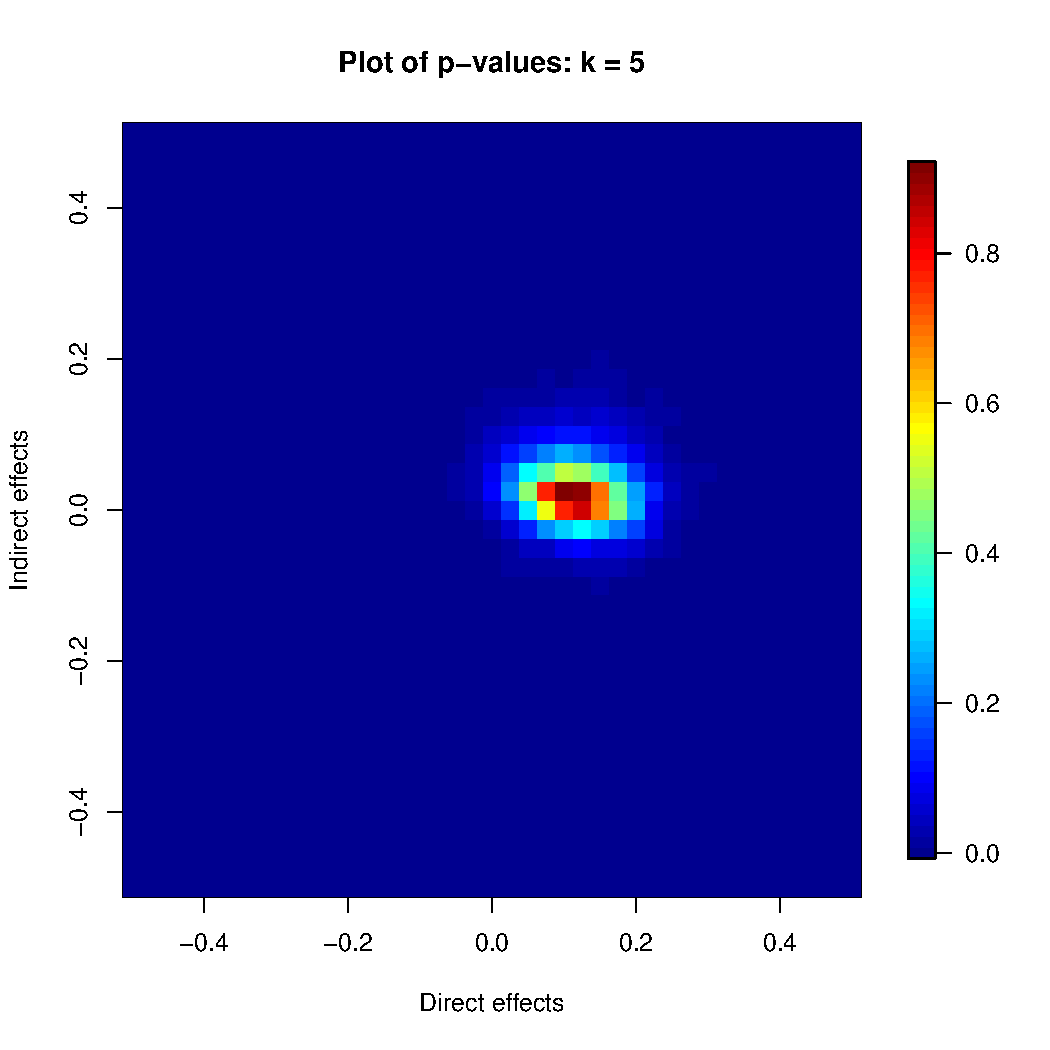
\includegraphics[scale=0.45]{./images/pvalues_figure_5nn_Bergan.pdf} \\ 
	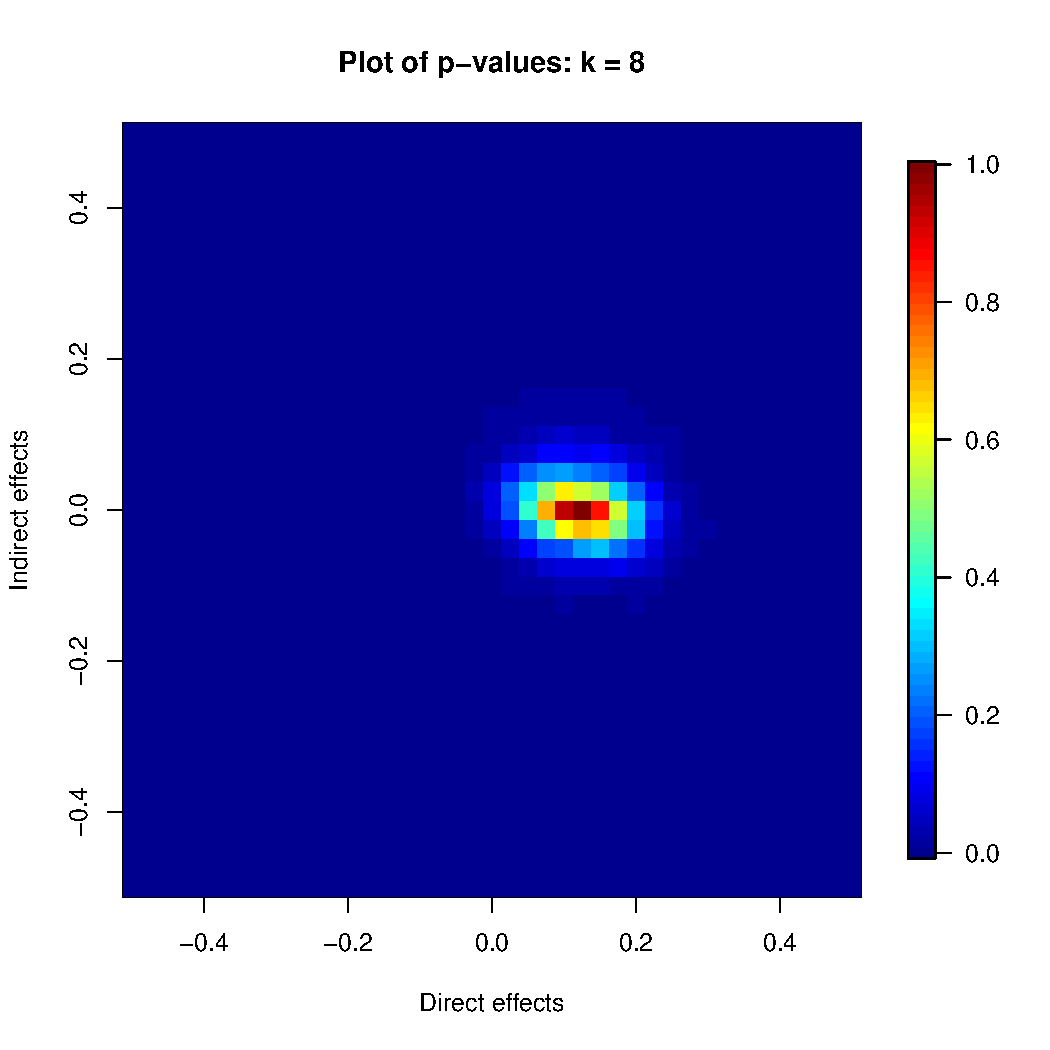
\includegraphics[scale=0.45]{./images/pvalues_figure_8nn_Bergan.pdf} &
	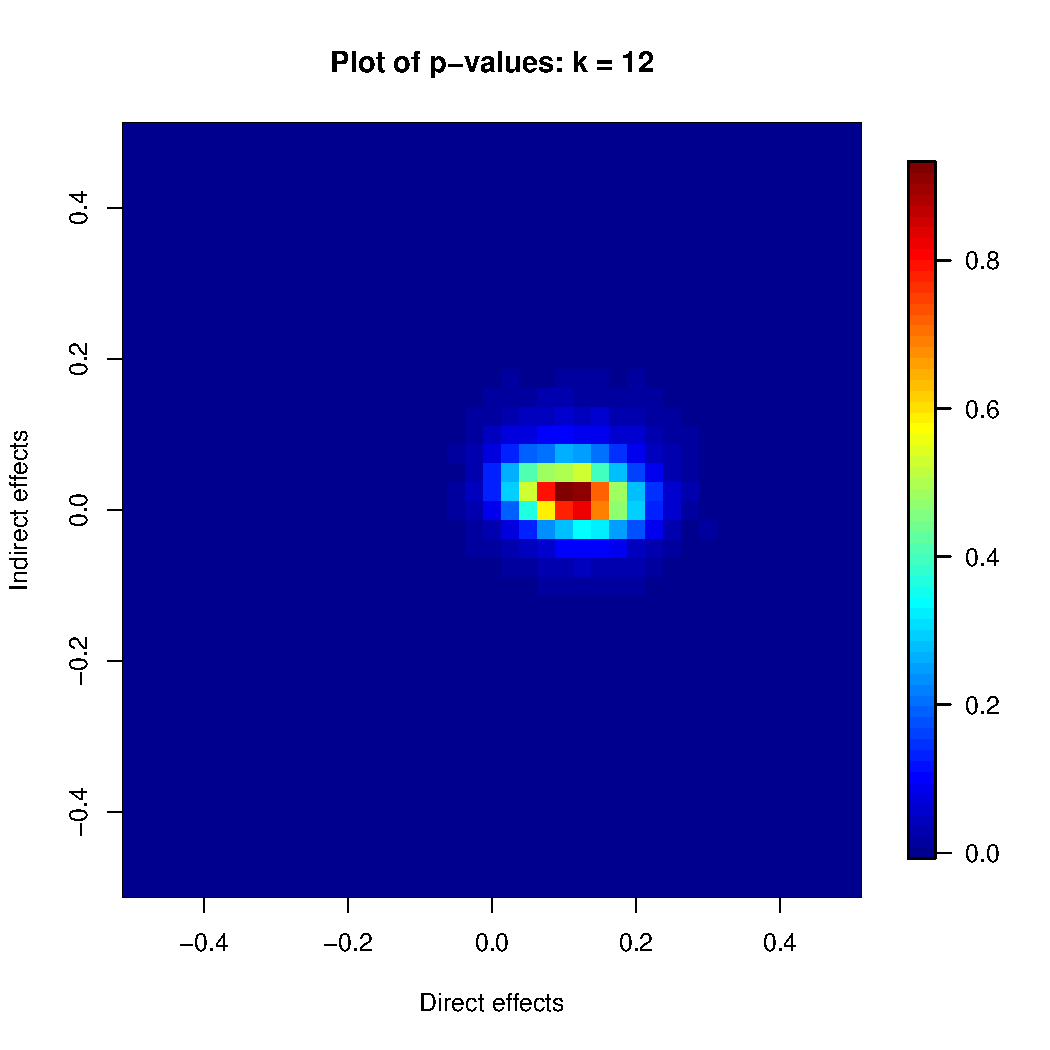
\includegraphics[scale=0.45]{./images/pvalues_figure_12nn_Bergan.pdf} \\ 
	\end{tabular}
	\caption{p-values: k-nearest neighbors for \citet{bergan2015call} data}
\end{figure}



\section{Network plots}

\begin{figure}
\centering
\begin{tabular}{cc}
{\bf Geographic Network} & {\bf Committee Network (>1 in common)}\\
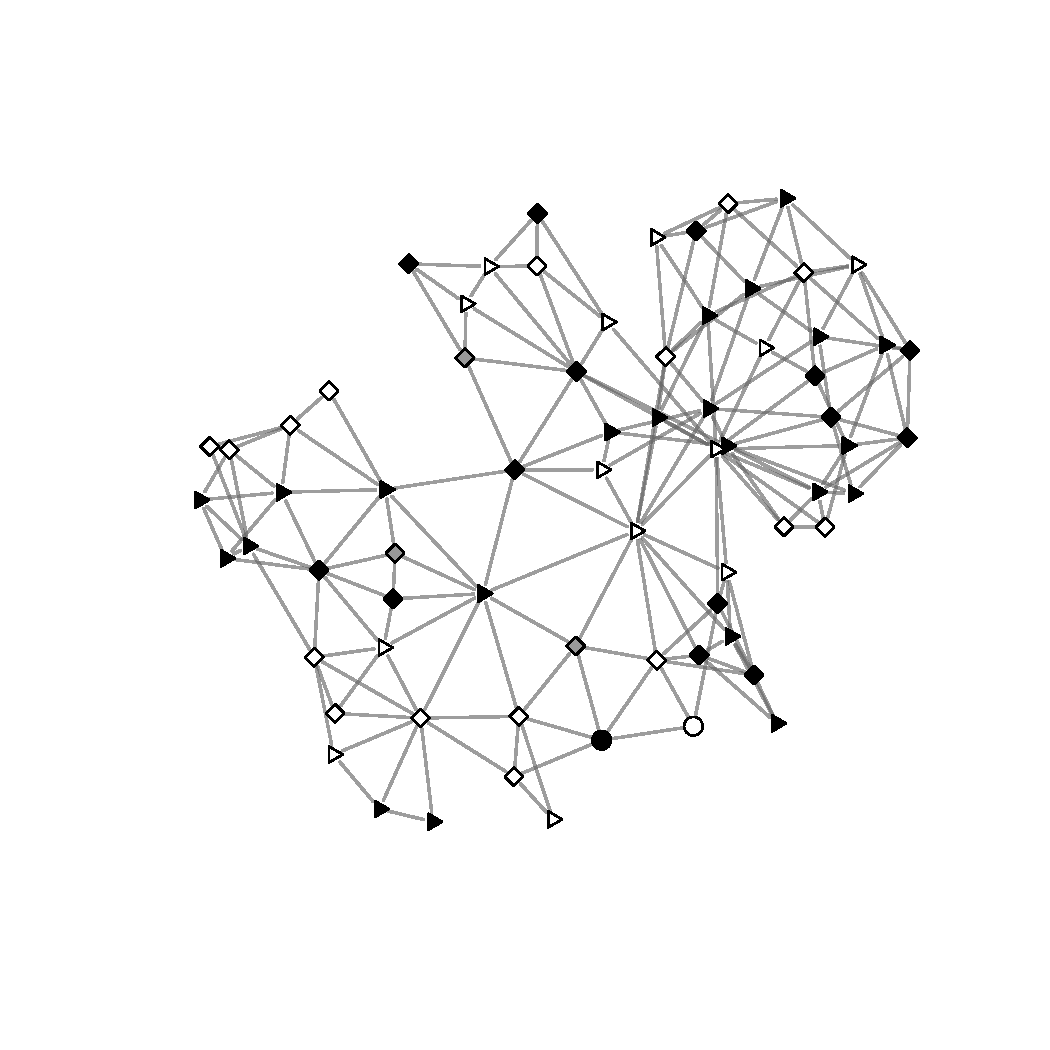
\includegraphics[scale=.55, clip=true,trim =2cm 2cm 2cm 2cm ]{./images/coppock_geographic_net.pdf} & 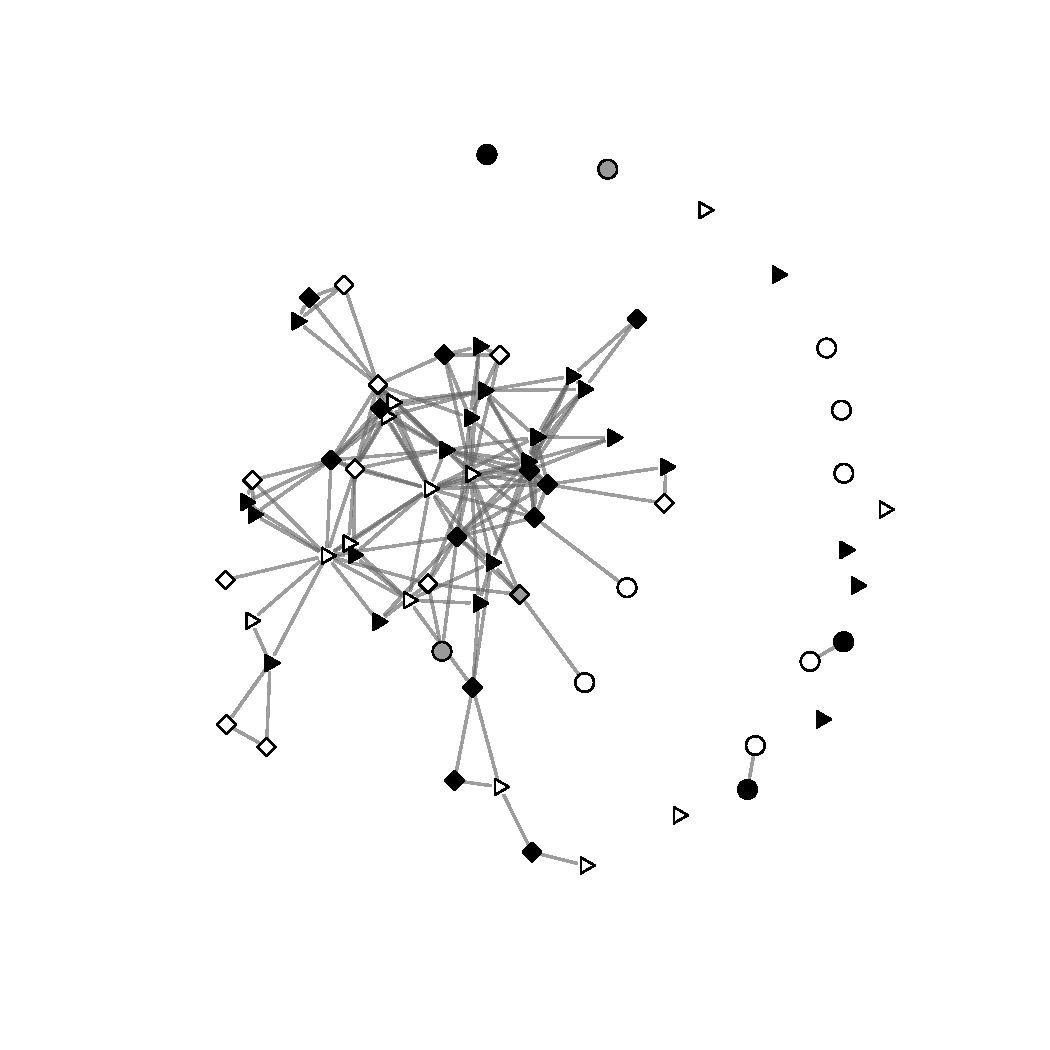
\includegraphics[scale=.55, clip=true,trim =2cm 2cm 2cm 2cm]{./images/nm_committee_net.pdf} \\ 
\end{tabular}
{\bf Ideological Network (top 5\%)} \\
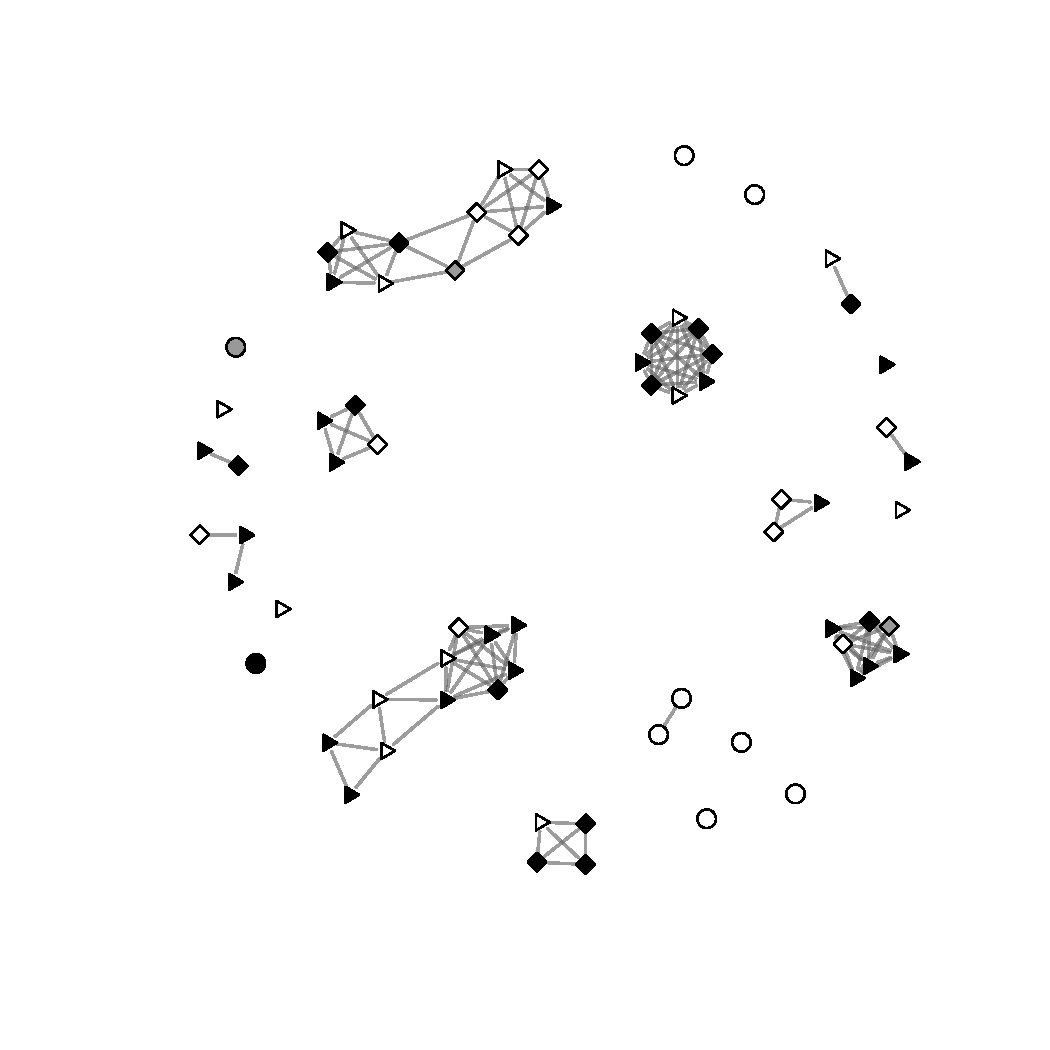
\includegraphics[scale=.55, clip=true,trim =2cm 2cm 2cm 2cm]{./images/coppock_ideological_net.pdf}
\caption{Different networks among New Mexico legislators. Colors denote outcome: black means voted with district, gray means abstained, white means voted against. Shape denotes treatment status. Triangles are treated. Squares are adjacent to treated. Circles are isolated from treatment}
\label{figure: nh-nets}
\end{figure}


\section{Appendix}
\subsection{Appendix 1A}

In this section, we will look at user-defined R-functions that replicate the \citet{bowers2012reasoning} methodology. This contains four steps:

\begin{itemize}
\item A function to transform the observed outcomes into potential outcomes for any treatment assignment w
\item A function to separate the hypothesized treatment effect
\item A function to calculate test statistic
\item A function to calculate the p-value.
\end{itemize}

The results from the ks.test function in R for calculating Kolmogorov-Smirnoff test statistic are verified with that in Footnote 12 of the paper.


\textbf{Function 1: calculating potential outcomes}

\begin{lstlisting}[language=R]
set.seed(132)
library(doParallel)
library(foreach)
library(kSamples)
library(network)
library(permute)

#### Potential outcomes ####

#### Transform uniformity trial outcome into observed outcome
unif.to.z <- function(z, S, y.0, beta, tau){
  # z: observed treatment assignment
  # S: adjacency matrix
  # y.0: outcome vector for uniformity trial
  # beta: growth curve parameter
  # tau: rate of growth parameter
  
  scalar <- as.vector(t(z)%*%S)
  spillover <- rep(NA, n)
  
  spillover <- beta + ((1-z) * (1-beta) * exp(-tau^2 * scalar))
  
  # This is equation 4
  h.y0.z <- spillover*y.0
}

#### Transform observed outcome into uniformity trial outcome
z.to.unif <- function(z, S, y.z, beta, tau){
  # z: initial treatment assignment
  # S: adjacency matrix
  # y.z: observed outcome vector
  # beta: growth curve parameter
  # tau: rate of growth parameter

  scalar <- as.vector(t(z)%*%S)
  spillover <- rep(NA, n)
  
  # Equation (3)
  spillover <- beta + ((1-z) * (1-beta) * exp(-tau^2 * scalar))
  
  # This is equation 5
  h.yz.0 <- (1/spillover)*y.z
}

#### Transform observed outcome into outcome for ANY other assignment w
z.to.w <- function(z, S, w, y.z, beta, tau){
  # z: initial treatment assignment
  # S: adjacency matrix
  # w: new treatment assignment
  # y.z: vector of outcomes for z
  # beta: growth curve parameter
  # tau: rate of growth parameter
  
  scalar.z <- as.vector(t(z)%*%S)
  scalar.w <- as.vector(t(w)%*%S)
  
  spillover.z <- rep(NA, n)
  spillover.z <- beta + ((1-z) * (1-beta) * exp(-tau^2 * scalar.z))
  
  
  spillover.w <- rep(NA, n)
  spillover.w <- beta + ((1-w) * (1-beta) * exp(-tau^2 * scalar.w))
  
  
  # Below is the actual function that transforms observed outcomes into potential outcomes
  # Equation (6)
  
  h.z.to.w <- (spillover.w / spillover.z) * y.z
}

#### Testing and p-value calculation ####

p.val <- function(z, y.z){
  
  cl <- makeCluster(4) #Setup for parallel computing
  registerDoParallel(cl)
    
  # Calculate the outcome vector after taking away the effect of treatment
  y.0 <- z.to.unif(z=z, S=S, y.z=y.z, beta=beta, tau=tau)
  
  # Calculate test statistic
  test.stat <- ks.test(y.0[z==1], y.0[z==0],
                       alternative = "g")$statistic
  sign <- noquote(strsplit(names(test.stat), NULL)[[1]])[3]
  if(sign=="+"){
    test.stat <- test.stat
  }else{
    test.stat <- test.stat*-1
  }  
  
  # Calculate a vector of test statistic using permutations
  results <- foreach (i = 1:perms) %dopar%{
    require(permute)
    perm.z <- z[sample(1:length(z),length(z),rep=F)]
    perm.test.stat <- ks.test(y.0[perm.z==1], y.0[perm.z==0],
                              alternative = "g")$statistic
    sign <- noquote(strsplit(names(perm.test.stat), NULL)[[1]])[3]
    
    if(sign=="+"){
      return(perm.test.stat)
    }else{
      return(perm.test.stat*-1)
    }
  }
  stopCluster(cl)
  
  # A vector of test statistics
  all.test.stat.vals <- unlist(results)
  
  # Calculating p-value
  pval <- sum(all.test.stat.vals > test.stat)/perms
  return(pval)
}
\end{lstlisting}


\subsection{Appendix 1B}

Below code replicates the \citet{coppock2014information} results using the framework setup in the Bowers replication code
(Version before final corrections by BD)

\begin{lstlisting}[language=R]

setwd("~/Dropbox/professional/Research/Active/causalityinnetworks-agenda/Interference_in_Field_Experiments/Analysis/coppock_replication_data/") # BD

rm(list=ls())
set.seed(312)

library(doParallel)
library(fields)
library(foreach)
library(kSamples)
library(network)
library(permute)
library(wnominate)


#### Read the original Butler and Nicketson data
#### This is the New Mexico dataset

data <- read.table("nm.replication.tab", sep="\t", header=TRUE)

z <- data$treatment #observed treatment
y.z <- data$sb24 #observed outcome
n <- length(y.z) #number of observations
t <- length(z[z==1]) #number of treated units
perms <- 10000 #number of permutations to use in generating expected exposure
perms.test <- 1000 #number of permutations used in testing


#### Generate Similarity Scores (this code taken from CoppockJEPS_datapreparation.R)

nmhouse2008 <-read.csv("CoppockJEPS_rollcalldata.csv")
bills <- data.frame(nmhouse2008[5:21])

## Nominate Scores

bills_nona <- bills
bills_nona[bills_nona==99] <- NA
rollcalls <- rollcall(bills_nona)
nominate_scores <- wnominate(rollcalls, polarity=c(1, 2), minvotes=10)
dwnom_scores <- nominate_scores$legislators$coord1D

get.similarity <- function(x, y){
  return((2-abs(x-y))/2)
}


## Create an adjacency/similarity matrix using ideology
S.ideo <- matrix(NA, ncol=70, nrow=70)
for (i in 1:70){
  for (j in 1:70){
    S.ideo[i,j] <- get.similarity(dwnom_scores[i], dwnom_scores[j])
  }
}
diag(S.ideo) <- 0
S.ideo[is.na(S.ideo)==T] <- 0


#### Generate expected exposure
perm <- replicate(perms, z[sample(1:length(z),length(z),rep=F)])

expected.exp0 <- rep(0, n)
expected.exp1 <- rep(0, n)

for(p in 1:ncol(perm)){
	zp <- perm[,p]
	for(i in 1:n){
		if (zp[i] == 1){
				expected.exp1[i] <- expected.exp1[i] + sum(S.ideo[i,-i]*zp[-i])
			}
			else{
				expected.exp0[i] <- expected.exp0[i] + sum(S.ideo[i,]*zp)
			}
	}
}
num_treat <- apply(perm,1,sum)
num_control <- apply(1-perm,1,sum)
expected.exp1 <- expected.exp1/num_treat
expected.exp0 <- expected.exp0/num_control


#### Generate expected and net exposure
#### This is the spillover effect model

indirect.treatment <- function(permutation, adj.mat){ #any treatment assignment vector and adjacency matrix can be used
  # permutation: can be the initial treatment assignment or a permutation
  raw.exp <- rep(NA, n)
  for (i in 1:n){
    raw.exp[i] <- sum(adj.mat[i,]*permutation)
    }
  
  net.exp <- raw.exp - (permutation*expected.exp1 + (1-permutation)*expected.exp0)
  standard.exp <- (net.exp - mean(net.exp))/sd(net.exp) #this is the spillover or indirect effect
  return(standard.exp)
}


#### We now model the uniformity trial transformation

z.to.unif <- function(outcome, beta1, beta2, permutation, adj.mat){
  # outcome: vector of direct treatment outcomes
  # beta1: direct treatment effect parameter
  # beta2: indirect treatment effect parameter
  # permutation: vector of a permutation of z (can be z itself)
  # adj.mat: adjacency matrix
  
  exposure <- indirect.treatment(permutation, adj.mat)
  # This is equation 5
  h.yz.0 <- outcome - (beta1*permutation) - (beta2*exposure)
  return(h.yz.0)
}


#### Testing and p-value calculation

beta1s <- seq(from=-.7, to=0.2, by=.025)
beta2s <- seq(from=-.7, to=0.2, by=.025)

pvals <- matrix(NA, length(beta1s), length(beta2s))

cl <- makeCluster(4) #Setup for parallel computing
registerDoParallel(cl)

pvalues.ideology <- foreach (i = 1:length(beta1s)) %do% {
  abc <- foreach (j = 1:length(beta2s)) %do% {
    
    # Calculate the outcome vector after taking away the effect of treatment
    y.0 <- z.to.unif(outcome = y.z, beta1 = beta1s[i], beta2 = beta2s[j], permutation = z, adj.mat = S.ideo)
    
    # Calculate observed test statistic
    exposure <- indirect.treatment(permutation = z, adj.mat = S.ideo)
    test.stat <- sum((lm(y.0 ~ z + exposure, na.action = na.omit)$resid)^2)
    
    # Calculate a vector of test statistic using permutations
    
    results <- foreach (k = 1:perms.test) %dopar% {
      require(permute)
      perm.z <- z[sample(1:length(z),length(z),rep=F)] #Each time we sample a permutation of z
      perm.y.0 <- z.to.unif(outcome = y.z, beta1 = beta1s[i], beta2 = beta2s[j], permutation = perm.z, adj.mat = S.ideo)
      perm.exposure <- indirect.treatment(permutation = perm.z, adj.mat = S.ideo)
      
      perm.test.stat <- sum((lm(perm.y.0 ~ perm.z + perm.exposure, na.action = na.omit)$resid)^2)
      }
    
    
    # A vector of test statistics
    all.test.stat.vals <- as.numeric(unlist(results))
    
    # Calculating p-value
    pval <- sum(all.test.stat.vals < test.stat)/perms.test
  }
  as.numeric(unlist(abc))
}

stopCluster(cl)

for (i in 1:length(beta1s)){
  pvals[i,] <- unlist(pvalues.ideology[i])
}

pvals


## Creating a plot
image.plot(beta1s, beta2s, pvals,
           main = "Plot of p-values", xlab = "Direct effects", ylab = "Indirect effects")

pdf("pvalues_figure.pdf")
image.plot(beta1s, beta2s, pvals,
           main = "Plot of p-values",
           xlab = "Direct effects", ylab = "Indirect effects")
dev.off()


\end{lstlisting}


%===================References======================
\clearpage
\bibliographystyle{apsr}
\bibliography{cause_and_networks}




\end{document}
